\clearpage
\subsection{Software}

\begin{figure}[ht]
    \begin{center}
        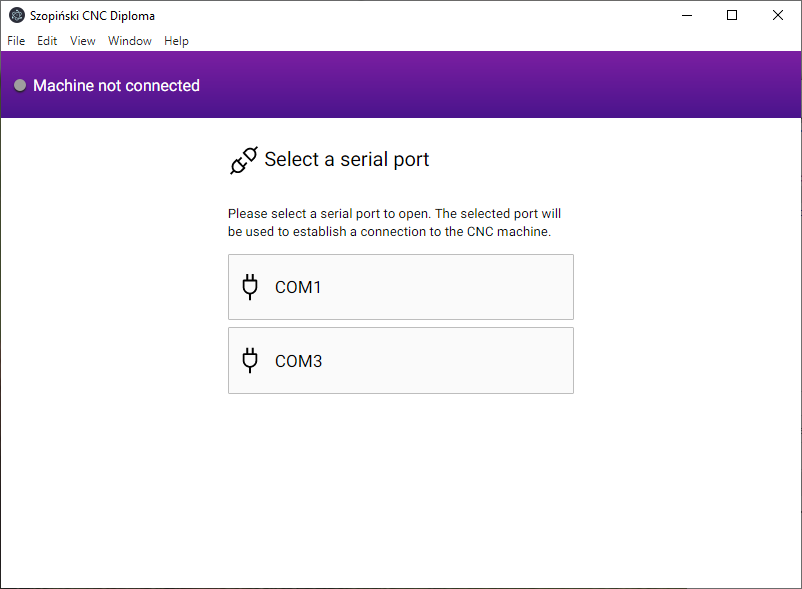
\includegraphics[width=0.75\linewidth]{serialselect}
        \caption{Serial port selection screen of the control software.}
        \label{serialselect}
    \end{center}
\end{figure}

The control software is implemented using Electron, a framework for writing
desktop applications using web technologies. This allows it to present an
elegant, modern user interface while retaining the ability to perform low-level
operations such as serial communication. It also makes it easy to achieve
cross-platform compatibility.

The following frameworks, packages and tools were used to create the
application:
\begin{itemize}
    \item Yarn, a combined package manager and project manager. Used for
    managing dependencies and launching build utilities.
    \item Webpack, a module bundler. Needed to compile the project into a
    compact set of files suitable for consumption by Electron.
    \item React, a framework for building user interfaces. It introduces a
    system of components and a mechanism to coordinate the flow of information
    within the application.
    \item React Redux, a library for managing the global application state.
    Facilitates handling events which impact multiple unrelated parts of the
    user interface.
    \item React Router, a library to handle screen navigation.
    \item Node SerialPort, a JavaScript wrapper around the operating system's
    serial interface.
    \item Sass, a dialect of CSS which introduces a hierarchical structure.
    \item ESLint, a code analysis tool for detecting errors and enforcing code
    style.
\end{itemize}
